\documentclass[12pt]{article}
\usepackage{geometry}
%\usepackage{times}
\geometry{a4paper, left=1in, right=1in, bottom=1in, top=1in}
\usepackage{authblk}
\usepackage{fancyhdr}
\usepackage{graphicx}
\usepackage{tabularx}
\usepackage{colortbl}
\usepackage{tabularx}

%define vars
\newcommand{\tit}{Intall Abaqus 2017 on a Linux System}
\newcommand{\ifp}{\textit{InstallationFileFolder}}
\newcommand{\cmd}[1]{
    \leavevmode{\parindent=0.05\textwidth\indent
    \begin{tabular}{>{\columncolor[gray]{0.8}}p{0.95\textwidth}}
        #1
    \end{tabular}
    }
}

%Paragraph
\setlength{\parindent}{0pt}
\renewcommand{\baselinestretch}{1.3}
\setlength{\parskip}{12pt}

%Title page
\title{
\includegraphics[height=1in]{Figures/NUIG_Logo.jpg}\\ \tit}
\author[1]{Yadong Jiang}
\affil[1]{College of Engineering and Informatics, National University of Ireland Galway}
\date{}

%Header and footer
\pagestyle{fancy}
\fancyhf{}
\lhead{
\includegraphics[height=0.5in]{Figures/NUIG_Logo.jpg}}
%\rhead{Yadong Jiang}
\rhead{\tit}
\setlength{\headsep}{0.5in}
\rfoot{Page \thepage}

%Tabular
\def\arraystretch{1.5}
\begin{document}
\maketitle

\newpage

\section*{Description}
This document aims to guide users to install and run Abaqus 2017 on a Linux machine. Table \ref{tb-1} summarizes the installation environments used in this guidance. Although Ubuntu is specified in the table, this instruction file is also suitable for installation of Abaqus on other Linux distributions (e.g. Archlinux, Fedora, etc.). The Linux desktop environment is not required. All installation steps are completed in terminal. Thus, this document is also suitable for users who want to install and run Abaqus on a Linux server remotely via SSH connection. Furthermore, if you want to install other version of Abaqus, you can still follow the methods given by this guide. But it should be highlighted that the administration right is required to complete the installation.

\begin{table}[h!]
\caption{Environments of Installation}
\begin{center}
\begin{tabular}{l l}
    \hline
    Linux Distribution: & Ubuntu 14.04.4 LTS (64 bits)\\
    \hline
    Linux desktop environment: & N/A \\
    \hline
    Administration Right: & Yes \\
    \hline
    Abaqus version: & Abaqus 2017 (64 bits) \\
    \hline
\end{tabular}
\end{center}
\label{tb-1}
\end{table}

\section*{Prerequirments}
\subsection*{Installation Files}
The Abaqus installation files should be transferred to the Linux machine. In this document, the root path of the installation files is marked \ifp. It should be noted that the \ifp\ \textbf{should not contain any ``space''}.

To avoid any permission issues, the permission of \ifp should be modified so that every user read/write/execute the installation files. To achieve this, simply run the following command in terminal.

\cmd{sudo chmod -R 777 \ifp}

\subsection*{Install Required Packages}
The Linux Abaqus installation program is based on ksh and the FLEXNET requires the lsb-core. The two packages should be installed before the installation of Abaqus by the following command:

\cmd{sudo apt-get install ksh lsb-core}

It should be noted that ``apt-get'' is the package handling utility of Ubuntu. If you are working with other Linux distribution, the command to install packages may vary.

\subsection*{Disguise Your Linux Distribution}
When the Abaqus installation program starts, it will check your Linux release name. If your Linux distribution is not ``Red Hat Enterprise Linux Server'', ``Red Hat Enterprise Linux Client'', ``Red Hat Enterprise Linux Workstation'', ``Cent OS''or ``Suse Linux'', the program will pop out error and exit, as shown in Figure \ref{fig-1}.

\begin{figure}[h!]
\begin{center}
    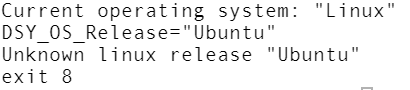
\includegraphics[width=0.5\textwidth]{Figures/UnknowLinux.png}
\end{center}
\caption{Unknown linux release}
\label{fig-1}
\end{figure}

To avoid this error, you have to disguise your Linux distribution as one of the aforementioned release names. The Abaqus installation program calls a script named ``Linux.sh'' to detect your Linux release name. You have to change the line ``DSY\_OS\_Release=`lsb\_release --short --id |sed 's/ //g'`'' to ``DSY\_OS\_Release=``CentOS'''', as shown in Figure \ref{fig-2}. By doing this, the installation program will detect your Linux release name as ``'Cent OS'.

\begin{figure}[h!]
\begin{center}
    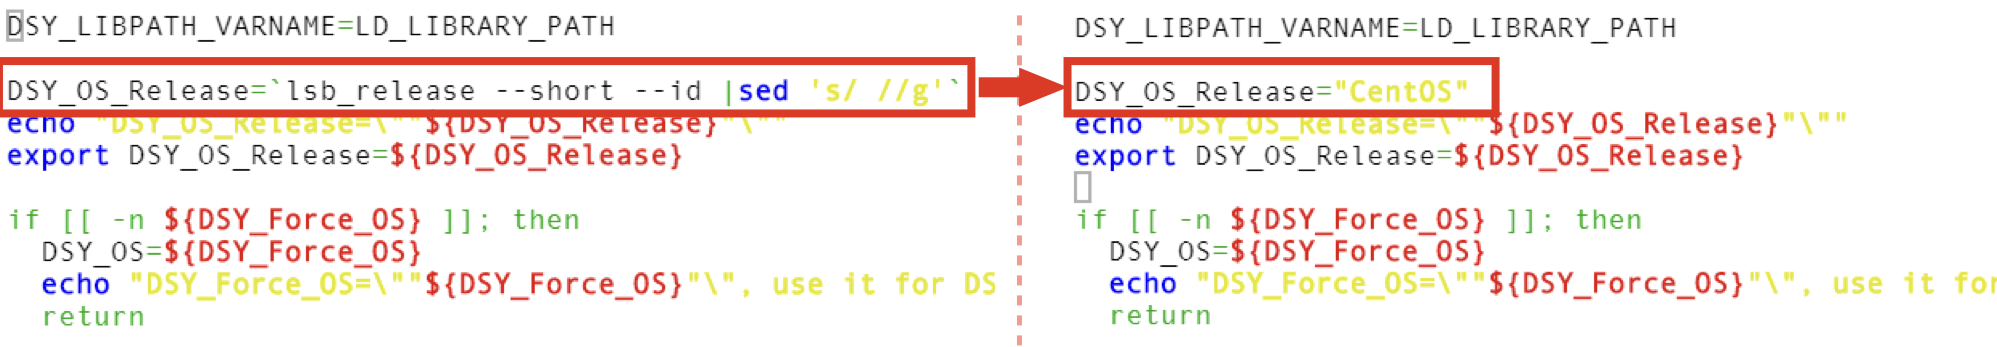
\includegraphics[width=\textwidth]{Figures/FakeLinux.png}
\end{center}
\caption{Change the ``Linux.sh'' file}
\label{fig-2}
\end{figure}

There are eight ``Linux.sh'' scripts in the \ifp, you need to modify all the eight files. The folders which contain the scripts are listed in Table \ref{tb-2}.

\begin{table}[h!]
\caption{Folders which contain the ``Linux.sh'' files}
\begin{center}
\begin{tabular}{l}
    \hline
    \ifp/1/inst/common/init \\
    \hline
    \ifp/1/SIMULIA\_Documentation/AllOS/1/inst/common/init \\
    \hline
    \ifp/2/SIMULIA\_FLEXnet\_LicenseServer/Linux64/1/inst/common/init \\
    \hline
    \ifp/2/SIMULIA\_AbaqusServices/Linux64/1/inst/common/init \\
    \hline
    \ifp/2/SIMULIA\_AbaqusServices\_CAA\_API/Linux64/1/inst/common/init \\
    \hline
    \ifp/2/SIMULIA\_Abaqus\_CAE/Linux64/1/inst/common/init \\
    \hline
    \ifp/2/SIMULIA\_Tosca/Linux64/1/inst/common/init \\
    \hline
    \ifp/3/SIMULIA\_Isight/Linux64/1/inst/common/init \\
    \hline
\end{tabular}
\end{center}
\label{tb-2}
\end{table}

\section*{Installation}
To start the installation program, the following command should be executed:

\cmd{\ifp/1/StartTUI.sh}

This command will start a installation program in terminal. Alternatively, if you have Linux with Desktop Environment installed, you can call the following command to start the installation program with a GUI.

\cmd{\ifp/1/StartGUI.sh}

When the installation program started, you can selected and install different components.



\begin{figure}[h!]
    \label{fig-3}
    \begin{center}
        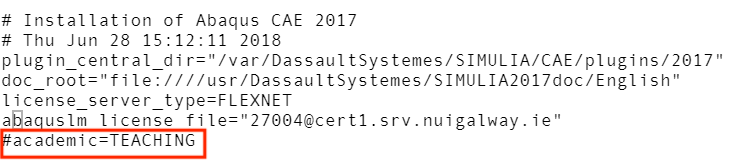
\includegraphics[width=\textwidth]{Figures/Custom_v6.png}
    \end{center}
    \caption{Change the license setting in the ``custom\_v6.env'' file}
\end{figure}

\section*{Start Abaqus}

\end{document}